\documentclass[11pt]{article}
\usepackage[a4paper,margin=1in]{geometry}
\usepackage{amsmath,amssymb,booktabs,array,graphicx,float}
\usepackage[T1]{fontenc}
\usepackage{lmodern}
\usepackage{microtype}
\usepackage{hyperref}
\usepackage{natbib}
\usepackage{enumitem}
\hypersetup{colorlinks=true,linkcolor=blue,citecolor=blue,urlcolor=blue}
\newcommand{\HSIC}{\operatorname{HSIC}}
\newcommand{\MMD}{\operatorname{MMD}}
\newcommand{\dcov}{\operatorname{dCov}}
\newcommand{\E}{\mathbb E}
\newcommand{\Cov}{\operatorname{Cov}}
\newcommand{\one}{\mathbf 1}
\title{Hermite rank and memory sums shape kernel-test size under long memory}
\author{Exploratory manuscript draft}
\date{23 October 2026}

\begin{document}
\maketitle

\begin{abstract}
We make three contributions to understanding kernel tests under long memory. First, controlled null experiments map how rejection varies with memory, transformation, sample size, and critical-value rule. At a nominal $5\%$ level and $n=2000$, split-sample maximum mean discrepancy (MMD) rejects 271 of 1,000 stationary fractional Gaussian noise (fGn) null series ($27.1\%$) at $H=0.8$ with uncentred wild multipliers. The Hilbert--Schmidt independence criterion (HSIC) rejects 184 of 2,000 independent fGn pairs ($9.2\%$) at $H_X=H_Y=0.7$ with subsampling. Persistent covariance changes the scale of kernel features, while a rule based on shorter dependence can miss that change. Second, a Hermite-rank calculation separates the rank-one split-MMD mechanism from the product-covariance mechanism of independence tests and identifies $H_X+H_Y=1.5$ as an organizing axis, without deriving a critical-value law. Third, a Nasdaq stock-duration study probes these rules in market data: at $n=2000$, HSIC shifts reject $3.4\%$--$5.6\%$ and subsampling $7.2\%$--$10.2\%$ across four 500-pair cells. The stock processes' independence is unverified, so those fractions are descriptive.
\end{abstract}

\noindent\textbf{Keywords:} long-range dependence; kernel tests; Hermite rank; MMD; HSIC; distance covariance; market microstructure.

\section{Introduction}
This paper makes three contributions for machine-learning tests on ordered data. First, it measures false-alarm rates for split MMD, HSIC, and distance covariance under known nulls. At a nominal $5\%$ threshold and $n=2000$, split MMD rejects 271 of 1,000 stationary fGn null series ($27.1\%$) at $H=0.8$ with uncentred wild multipliers. HSIC rejects 184 of 2,000 independent fGn pairs ($9.2\%$) at $H_X=H_Y=0.7$ with subsampling. Persistent covariance in the tested features changes their scale; the critical-value rule controls how much of that dependence is represented. Second, a Hermite-rank calculation explains why a one-series split and an independent two-series product have different covariance rates. It suggests a memory-sum axis but does not prove the tests' null laws. Third, separated Nasdaq stock-trade windows probe the rules where process independence is unknown.

Machine-learning systems use MMD to check distribution shift and HSIC to check dependence between paired representations. Both often receive observations ordered in time. The controlled grid varies memory, transformation, sample size, and critical-value rule so that each reported false-alarm rate has a specified generator and reference distribution.

The technical difficulty is that long memory persists after many observations have passed. A series of length $n$ then carries less information than $n$ independent draws. A rank-one feature retains the slow covariance decay of its Gaussian driver, while an even rank-two transform can reduce it. A critical-value rule that uses short windows or short multiplier correlations can represent a different amount of that dependence from the full statistic. Our experiments measure the resulting rejection rates rather than assume that a familiar rule remains valid.

The two kernel tasks have different nulls and leading terms. Split MMD compares the first and second halves of one stationary series. HSIC and distance covariance test independence between two aligned series. The rank-one split-MMD feature can change rate for any $H>1/2$. For independent rank-one factors, the leading cross-series covariance is summable when $H_X+H_Y<3/2$. This calculation motivates the simulation grid. It does not supply the critical values used by MMD or HSIC.

The critical-value rule must therefore be part of a reported result. At $H_X=H_Y=0.7$ and $n=2000$, HSIC rejects $9.2\%$ with subsampling, $7.35\%$ with wild multipliers, and $5.45\%$ with circular shifts on the same independent-fGn cell. The wild-multiplier rule already rejects $6.5\%$ when both series have $H=0.5$. Table~\ref{tab:rules} places these baseline and memory-grid rates beside the dependence each rule retains or discards.

Finally, we use separated trade-duration windows from Nasdaq stocks AAPL, MSFT, and NVDA as an applied boundary test for market microstructure. Each window stays inside one regular trading session, and paired days are at least 20 trading days apart. The gap does not establish process independence. We report these rejection fractions as descriptive placebos, not as false-alarm rates or evidence for one duration mechanism.

\section{Theory and predictions}\label{sec:theory}
\subsection{Memory and rank}
Write the autocovariance of a stationary Gaussian driving series as
\begin{equation}\label{eq:memory}
\rho(k) \sim c k^{-D}L(k),\qquad D=2-2H,\quad 1/2<H<1,
\end{equation}
where $L$ varies slowly. If a centred transform $g(\xi_t)$ has Hermite rank $m$, its leading covariance term has order $\rho(k)^m$. Away from equality, $mD>1$ makes this term summable and motivates a conventional square-root-$n$ partial-sum regime. At $mD=1$, the slowly varying factor can determine summability. This scalar calculation does not give a kernel statistic's null law or critical value. Two-sample $U$-process theory under long memory is available in \citet{dehling2017twosample}.

For rank one, $D<1$ whenever $H>1/2$, so the sample mean converges more slowly than $n^{-1/2}$. For rank two, $2D=1$ at $H=3/4$. \citet{zhai2026ggmlong} give a related rank-two example for a different sample-covariance-based graphical-model statistic, under Gaussian linear-process assumptions and a coefficient-decay condition above $3/4$. Their theorem does not address MMD or HSIC.

\subsection{Two-sample MMD}
For one observed series $Z_1,\ldots,Z_n$, split at $n/2$ and compare the kernel mean embeddings of the halves:
\begin{equation}\label{eq:mmd}
\MMD_n^2=\left\|\frac{2}{n}\sum_{t\leq n/2}\phi(Z_t)
-\frac{2}{n}\sum_{t>n/2}\phi(Z_t)\right\|_{\mathcal H}^2.
\end{equation}
Under stationarity, the population embeddings of the two halves agree. A nonzero first Hermite coefficient of $\phi(G(\xi_t))$ gives their sample difference a rank-one leading term, suggesting nonstandard scaling for any $H>1/2$. An even transform such as $G(\xi)=\xi^2-1$ can remove that term and make rank two leading. These predictions motivate the MMD contrasts below; \citet{dehling2017twosample} do not directly give this statistic's full null law.

\subsection{Independence statistics}
For paired observations $(X_t,Y_t)$, empirical HSIC and distance covariance square a centred cross-dependence term. Schematically, its leading summand is
\begin{equation}\label{eq:cross}
 U_t=\{f(X_t)-\E f(X_t)\}\{g(Y_t)-\E g(Y_t)\}.
\end{equation}
If the \emph{two processes} are independent and the leading factors each have rank one, then $\Cov(U_0,U_k)$ factors into two long-memory covariances. Its leading decay is $k^{-(D_X+D_Y)}$. Summability suggests a crossover at
\begin{equation}\label{eq:sum}
D_X+D_Y=1 \quad\Longleftrightarrow\quad H_X+H_Y=3/2.
\end{equation}
For equal memories this gives $H=3/4$ in each series. Unequal pairs test whether the sum, rather than the larger individual $H$, organizes the finite-sample behaviour.

Betken and Dehling derive a limit for the empirical joint characteristic-function process under independent Gaussian-subordinated series; their corollary yields a distance-covariance limit. The Gaussian side requires \emph{both} memory exponents $D_X,D_Y>1/2$, corresponding to both $H$ values below $3/4$ \citep[Theorem 2.2(i) and Corollary 2.1(i)]{betken2021ldr}. Their non-central characteristic-function result above the crossover uses Gaussian identity transforms with $D_X+D_Y<1$ \citep[Theorem 2.2(ii) and Corollary 2.1(ii)]{betken2021ldr}. Their theorem does not settle a mixed pair with one $H>3/4$ but $H_X+H_Y<3/2$. Nor does it directly prove the same result for Gaussian-kernel HSIC. Equation~\eqref{eq:sum} is therefore a mechanism and an empirical organizing axis for our HSIC experiments, with a narrow proved neighbour for distance covariance.

\begin{table}[H]
\centering\small
\caption{Scope of the theory used to motivate the experiments. No cited result validates every implemented critical-value rule.}\label{tab:scope}
\begin{tabular}{@{}p{0.24\linewidth}p{0.31\linewidth}p{0.35\linewidth}@{}}
\toprule
Result & What it covers & What remains open here \\
\midrule
Hermite covariance calculation & Rate of a scalar transformed Gaussian mean or independent product feature & RKHS-valued split-MMD and HSIC limits; critical-value laws \\
\citet{betken2021ldr}, Thm.~2.2 and Cor.~2.1 & Characteristic-function limit; distance-covariance corollary & Gaussian-kernel HSIC; mixed normal region; exact finite-sample rule below \\
\citet{betken2021ldr}, Thm.~2.4 & Subsampling for a statistic with a limit, under process and block conditions & Exact HSIC and dCov transfer; finite-sample size \\
\citet{chwialkowski2014wild} & Wild bootstrap under weak-dependence assumptions & Long-memory validity of the present multiplier rule \\
\bottomrule
\end{tabular}
\end{table}

The wild-bootstrap theory of \citet{chwialkowski2014wild} and the random-process HSIC work of \citet{chwialkowski2014random} use weak-dependence conditions that need not hold here. Betken and Dehling give a general subsampling result for a statistic with a nondegenerate limit under independent Gaussian-subordination and block-length conditions \citep[Theorem 2.4]{betken2021ldr}. Combined with their distance-covariance limit, it may cover restricted independent-fGn dCov cases after an exact check of the statistic and block rule. The theorem permits the offset $d_n=\lfloor0.1n\rfloor$, which the authors also use in simulations. It does not establish our HSIC critical-value rule: an HSIC null limit is missing, and our windows reuse bandwidths chosen from the full sample. Finite-sample size can still be poor. Other long-memory subsampling and self-normalized block results \citep{betken2018subsampling,bai2016snbs} likewise require conditions on the statistic. Block choice matters under Gaussian subordination \citep{zhang2022optimalblock}.

\section{Experimental design and reproducibility}\label{sec:methods}
All reported tests use a nominal $5\%$ rejection threshold. Under the simulated nulls, each rejection proportion estimates a false-alarm rate: the independence arms generate independent series, and the homogeneity arm splits one stationary series. For trade data, the process-independence null is unknown, so we report \emph{placebo rejection rates}. Wilson intervals describe counting uncertainty in simulation rates; they do not cover uncertainty about the model, kernel, or critical-value rule.

\begin{table}[H]
\centering\small
\caption{Study arms. A simulation cell's null is fixed by its generator; the stock placebo has an unverified process-independence null.}\label{tab:design}
\begin{tabular}{@{}p{0.19\linewidth}p{0.38\linewidth}p{0.16\linewidth}p{0.17\linewidth}@{}}
\toprule
Arm & Series and comparison & Sample size & Replications or pairs \\
\midrule
Initial MMD & Stationary fGn and transforms, split in halves & 500--4,000 & 1,000--2,000 \\
Initial independence & Independent fGn, subordinated and unequal-memory pairs & 500, 1,000, 2,000 & 2,000 per cell \\
EXP1 H5/E2 & MMD rule control and rank-one/two transforms & 500, 1,000, 2,000 & 1,000--2,000 \\
EXP1 E3 & Ten equal or unequal independent fGn pairs & 500, 1,000, 2,000 & 2,000 per cell \\
Stock placebo & Separated AAPL, MSFT, NVDA duration windows & 500, 1,000, 2,000 & 500 pairs per cell \\
Revision control & Independent $H=0.5$ fGn pairs; centred versus raw multipliers & 500, 1,000, 2,000 & 1,000 per cell \\
\bottomrule
\end{tabular}
\end{table}

We compared empirically centred Markov multipliers with raw multipliers on independent $H=0.5$ Gaussian pairs. The comparison isolates baseline rule error before interpreting long-memory cells; its selection criterion and full counts are in Appendix~\ref{sec:evidence}.

\subsection{Initial MMD and independence map}
The initial MMD arm applies Gaussian-kernel MMD to the first and second halves of fractional Gaussian noise (fGn), a bounded transform $2\Phi(\xi)-1$, $\operatorname{sign}(\xi)$, and a slow-mean-reversion comparison. In the latter, $Y_t=(1-\lambda)Y_{t-1}+\varepsilon_t$ with independent fGn innovations of $H=0.1$, $\lambda\in\{0.01,0.1\}$, and a burn-in of $\lceil10/\lambda\rceil$ observations. This is a discrete mean-reverting process driven by anti-persistent noise, not a claim of continuous-time fractional OU sampling. The fGn memory grid is $H\in\{0.5,0.6,0.7,0.75,0.8,0.9\}$. We compare wild-multiplier and sampling-window critical-value rules.

The independence arm compares Gaussian-kernel HSIC with a median-distance bandwidth, distance covariance, and Pearson correlation as a linear reference. Its generators include fGn, bounded and sign subordinations, unequal-memory pairs, and independent copies of the mean-reverting process just defined. Kernel sample sizes are $n\in\{500,1000,2000\}$; Pearson uses $T\in\{500,2000,8000\}$.

For HSIC and distance covariance, the wild rule used empirically centred block-Markov Rademacher multipliers with correlation $\exp(-k/\ell)$, $\ell=\lfloor\sqrt n\rfloor$, and 500 draws. The HSIC shift rule compared the observed alignment with circular shifts from $\lfloor0.1n\rfloor$ through $n-\lfloor0.1n\rfloor$. Subsampling used windows of length $\ell=\lfloor\sqrt n\rfloor$ and a cross-series offset $\lfloor0.1n\rfloor$. Pearson references used Newey--West (NW) and equal-weighted-cosine (EWC) long-run variance rules. These are implementation choices, not broad guarantees of validity.

The finite-sample HSIC statistic is $T_n=n^{-1}\sum_{i,j}K^c_{ij}L^c_{ij}$, where $K^c,L^c$ are empirically double-centred Gaussian Gram matrices and each bandwidth is the median of off-diagonal pairwise distances, with the implementation's positive-distance fallback for ties. The distance-covariance statistic replaces these Gram matrices with double-centred pairwise-distance matrices. Thus $T_n=nV_n$ for each biased $V$-statistic. For a multiplier draw $w$, the reference statistic is $n^{-1}w^\top(K^c\circ L^c)w$, or the analogous distance product, and its upper-tail $p$-value is $(1+\#\{b:T_b^*\geq T_n\})/(B+1)$. The same count rule compares zero-shift HSIC with permitted circular shifts. For each subsampling window, the code computes $T_{\ell}=\ell V_{\ell}$ and rejects when $T_n$ exceeds the empirical $95$th percentile of these window values. The generator is Davies--Harte fGn. These definitions describe the implementation, not an asymptotic guarantee.

\subsection{EXP1 rule checks, rank change, fine grid, and stock-trade data}
The simulation extension adds H5, E2, and E3. H5 compares five MMD multiplier variants at $H=0.5$ to isolate oversize present without long memory. E2 studies the even rank-two transforms $\xi^2-1$ and $|\xi|$, adds $H=0.55$, and compares multiplier lengths, two subsampling block rules, plug-in rate correction, and self-normalized versions. The self-normalized block statistic is $T_n^{\rm SN}=n\MMD_n^2/V_n$, where $V_n$ is the sum of squared deviations of RKHS partial sums from their within-half linear bridges, divided by $n^2$. Its critical value is the $95$th percentile of the same ratio calculated on every contiguous window of length $\lfloor n^{0.5}\rfloor$ or $\lfloor n^{0.7}\rfloor$. This ratio removes an unknown common scale under suitable conditions; it does not itself establish a valid rule for the present statistic. The exact $V_n$ and cell counts are given in Appendix~\ref{sec:evidence}.

E3 uses ten equal and unequal fGn pairs with $H_X+H_Y$ from $1.3$ to $1.7$. Each $n\in\{500,1000,2000\}$ cell has 2,000 replications. We plot rejection rates and adjacent-grid slopes directly, without fitting a breakpoint.

The applied arm uses Databento XNAS.ITCH trade records\footnote{Dataset and trade-schema documentation: \url{https://databento.com/datasets/XNAS.ITCH} and \url{https://databento.com/docs/schemas/trades}.} for AAPL, MSFT, and NVDA from January through June 2024. We keep regular-session trades from 09:30 to 16:00 New York time, sort by event timestamp and feed sequence, and collapse prints sharing an event timestamp. A positive gap between consecutive distinct timestamps is one intertrade duration. For each stock, we take its log duration in seconds and subtract the pooled mean log duration in its 15-minute clock bin. The cache also retains raw nanosecond gaps, event timestamps, day labels, and clock bins (Appendix~\ref{sec:evidence}).

A placebo pair takes random-start windows of 500, 1,000, or 2,000 consecutive durations, each wholly inside one trading day. Paired days are at least 20 trading sessions apart. The four pairings are AAPL--MSFT, AAPL--NVDA, MSFT--NVDA, and AAPL--AAPL. The same-stock pairing probes the sampling rule but does not establish independence. We draw 500 pairs in each of 12 cells and apply the same HSIC, distance-covariance, and Pearson implementations as in the simulated independence arm. Multiple pairs can reuse a day, and seasonal adjustment uses pooled data. The resulting rejection fractions are descriptive; they are not false-alarm estimates under a verified null.

\section{Results}\label{sec:results}
Table~\ref{tab:rules} compares the independence-test rules before separating their individual results. Baseline error is visible at $H_X=H_Y=0.5$, while the two memory-sum columns show what changes with persistent inputs. The last numeric column shows that rejection need not grow over $n=500$--$2000$ even when it is far above $5\%$.

\begin{table}[H]
\centering\footnotesize
\setlength{\tabcolsep}{4pt}
\caption{Independent-fGn false-alarm rates at nominal $5\%$. The first three numeric columns are percentages at $n=2000$ for equal-memory pairs with $(H_X,H_Y)=(0.5,0.5),(0.7,0.7),(0.8,0.8)$. $\Delta$ is the percentage-point change from $n=500$ to $n=2000$ at sum $1.6$. Each cell has 2,000 replications. Theory status refers to the exact rule used here.}\label{tab:rules}
\begin{tabular}{@{}lrrrrp{0.20\linewidth}p{0.23\linewidth}@{}}
\toprule
Rule & $H=.5$ & Sum 1.4 & Sum 1.6 & $\Delta$ & What it truncates & Theory for this rule \\
\midrule
HSIC wild & 6.5 & 7.4 & 8.9 & $-2.4$ & Multiplier memory beyond $\sqrt n$ lags & Weak-dependence theory only \\
HSIC shift & 5.0 & 5.5 & 5.7 & $-0.3$ & Shift offsets $<0.1n$; retains full series & No long-memory validity theorem here \\
HSIC sub & 5.6 & 9.2 & 19.7 & $-2.2$ & Observations outside $\sqrt n$ windows & HSIC limit and rule match open \\
dCov wild & 6.6 & 7.1 & 9.6 & $-2.2$ & Multiplier memory beyond $\sqrt n$ lags & Weak-dependence theory only \\
dCov sub & 5.3 & 10.6 & 23.0 & $-2.2$ & Observations outside $\sqrt n$ windows & Restricted dCov limit; block match open \\
Pearson NW & 5.8 & 8.2 & 13.3 & $-0.3$ & Covariance lags beyond fitted cutoff & Standard HAC theory excludes these cells \\
Pearson EWC & 6.1 & 6.0 & 8.5 & $+0.8$ & Cosine modes beyond $\lfloor0.4n^{2/3}\rfloor$ & Long-memory guarantee open \\
\bottomrule
\end{tabular}
\end{table}

\subsection{MMD rejection by rank and critical-value rule}
In the initial rank-one MMD experiment, rejection at the nominal $5\%$ level reaches about $12$--$19\%$ by $H=0.6$ and $44$--$71\%$ by $H=0.9$, depending on the process and critical-value rule. The observed increase starts near the low end of the tested grid, as the rank-one covariance calculation suggests. The grid does not identify a numerical breakpoint.

The H5 control shows why the bootstrap baseline matters. For Gaussian fGn at $H=0.5$ and $n=2000$, the old and published centred MMD multipliers reject $7.0\%$ and $7.2\%$ of null samples; independent and uncentred versions reject $5.3\%$ and $5.0\%$. At $n=500$, the old and centred rules reject about $9\%$. We use the on-size uncentred rule for the E2 memory comparison. These results concern the tested implementations and do not establish a general preference against centering.

E2 shows a different pattern for even rank-two transforms. With the uncentred wild multiplier at $n=2000$, rejection for $\xi^2-1$ is $5.0,5.9,4.2,5.2,6.4,11.3,22.8\%$ across the seven $H$ values from $0.5$ to $0.9$. The $|\xi|$ results have a similar shape, while rank-one references depart from nominal by $H=0.55$. Self-normalized block MMD changes less across the grid but still rejects about $6.0$--$8.5\%$ on fGn and $4.7$--$7.5\%$ on signs.

The single $H=0.7$ fGn shift-power cell at $n=2000$ gives $51\%$ alternative rejection for self-normalized MMD, compared with $76$--$87\%$ for conventional wild and subsampling rules at their implemented cutoffs. Their null rejection rates differ, so this is not a size-adjusted power comparison. Plug-in rate correction is often conservative and also rejects fewer alternatives in that cell.

\begin{figure}[H]
\centering
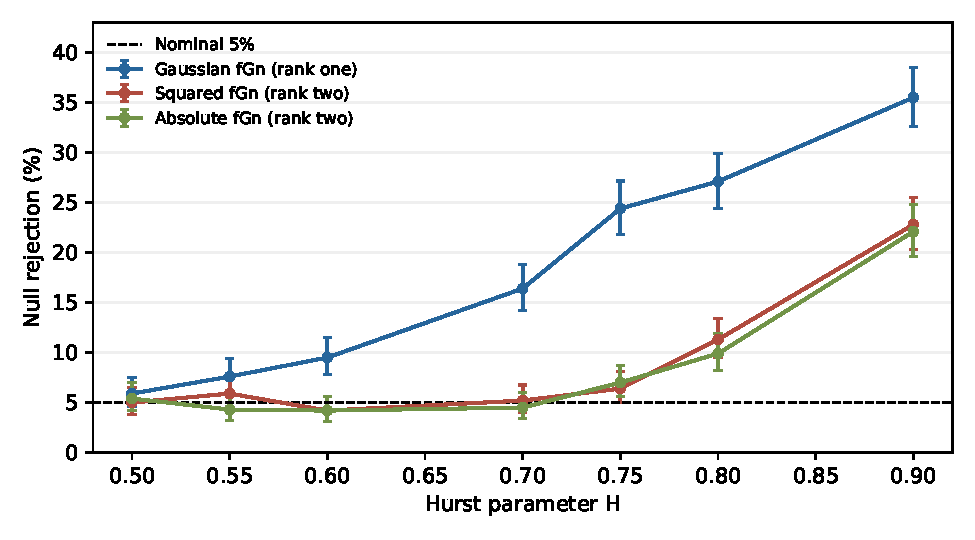
\includegraphics[width=0.83\linewidth]{figures/mmd_size.pdf}
\caption{MMD rejection under the stationary split-series null at $n=2000$, using the tested uncentred wild multiplier with length $\lfloor n^{0.5}\rfloor$. Points are saved E2 cell rates; bars are Wilson $95\%$ counting intervals from 1,000 replications. The lines compare process-specific finite-sample behaviour, not proved asymptotic thresholds.}\label{fig:mmd}
\end{figure}

\subsection{Independence-test rejection across memory pairs}
In the initial independence experiments, some HSIC, distance-covariance, and Pearson critical-value rules reject more sharply as $H_X+H_Y$ rises. The anticipated growth of kernel-test excess with $n$ above the candidate $1.5$ line is not consistent at $n\leq2000$: rates are often flat or fall, even in strong-memory cells (Table~\ref{tab:rules}). Across this grid, circular shifts give the most stable kernel-test size, while subsampling becomes strongly oversized at high memory.

E3 shows excess rejection even below the candidate $1.5$ line. At $(H_X,H_Y)=(0.7,0.7)$ and $n=2000$, HSIC and distance-covariance subsampling reject $9.2\%$ and $10.6\%$ of independent pairs. HSIC rejects $7.35\%$ with wild multipliers and $5.45\%$ with circular shifts; the linear NW and EWC references reject $8.15\%$ and $5.95\%$. HSIC subsampling stays near $9.2\%$ at all three sample sizes ($9.1,9.15,9.2\%$ at $n=500,1000,2000$). The wild-multiplier reference already rejects $6.45\%$ at $H=0.5$ and $n=2000$, so its below-line excess includes baseline rule error.

The unequal pair $(0.55,0.85)$ has kernel-test rates similar to the equal pair $(0.7,0.7)$. The memory sum is therefore a useful coordinate for this grid. A mixed-memory limit theorem for these exact tests remains open.

Figure~\ref{fig:ind} puts the critical-value rules on the same memory-sum axis. At $1.4$, subsampling is already oversized and circular shifts are near nominal. The algebraic $H_X+H_Y=3/2$ balance helps read the curves, but no common rejection boundary appears. Figure~\ref{fig:slope} displays adjacent-grid changes without estimating a breakpoint. Those local slopes are descriptive and sensitive to Monte Carlo variation and grid spacing.

\begin{figure}[H]
\centering
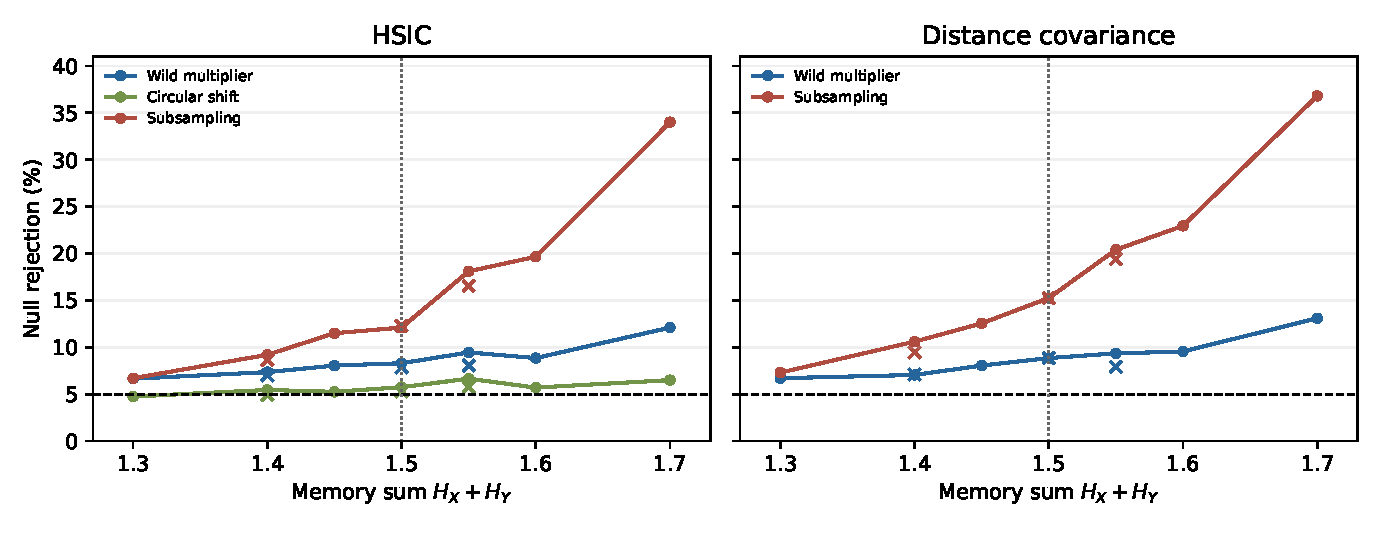
\includegraphics[width=\linewidth]{figures/independence_size.pdf}
\caption{E3 null rejection at $n=2000$ for independent fGn pairs. Connected circles are equal-memory pairs; crosses are unequal pairs. The horizontal dashed line is the nominal $5\%$ rate and the vertical dotted line marks the candidate sum $H_X+H_Y=1.5$. Each point has 2,000 replications. No line is a proved rejection boundary.}\label{fig:ind}
\end{figure}

\begin{figure}[H]
\centering
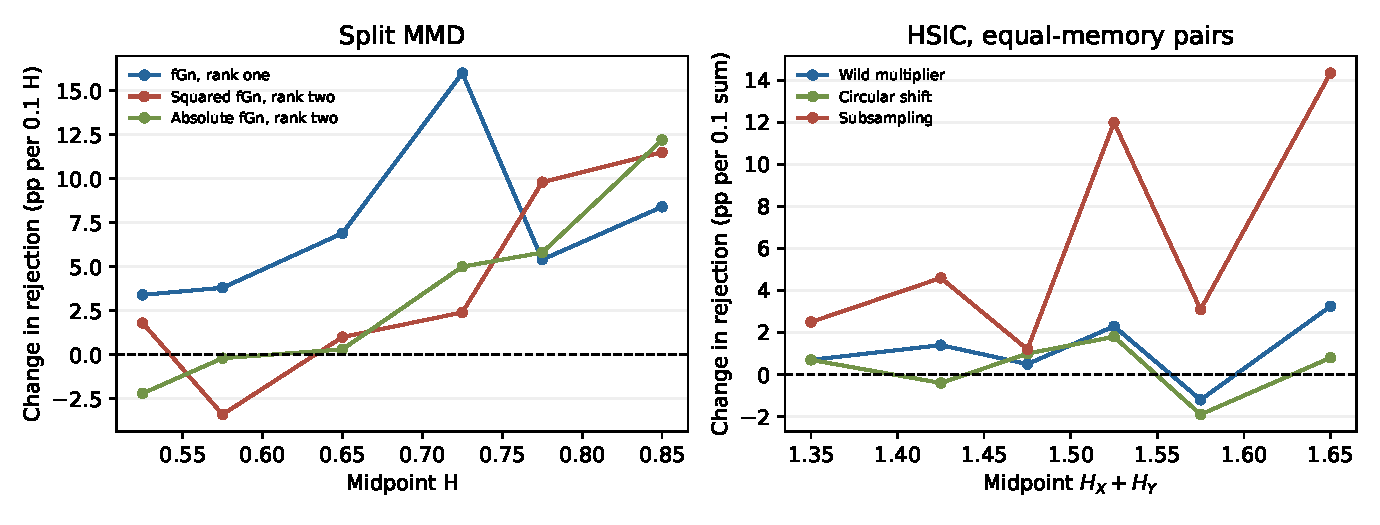
\includegraphics[width=\linewidth]{figures/size_slopes.pdf}
\caption{Adjacent-grid changes in null rejection at $n=2000$. Left: split MMD under the uncentred wild rule, measured in percentage points per $0.1$ increase in $H$. Right: HSIC on equal-memory independent pairs, measured per $0.1$ increase in $H_X+H_Y$. Points sit at interval midpoints. These finite differences are descriptive, depend on grid spacing and Monte Carlo error, and do not estimate a change point.}\label{fig:slope}
\end{figure}

In a separate $H=0.5$ control, removing empirical centering moves the HSIC and distance-covariance multiplier rules from oversize to undersize. It does not provide a uniformly better replacement. The stock placebo therefore uses the original centred multipliers. Full paired counts and the rule-selection criterion are in Appendix~\ref{sec:evidence}.

\subsection{Stock trade-duration placebo pairs}\label{sec:real}
The six-month extraction yielded 124 trading days for each stock and 9.68 million AAPL, 6.57 million MSFT, and 14.21 million NVDA positive intertrade durations. Each stock has observations in all 26 clock bins. The date separation and within-day window construction prevent the two sampled windows from overlapping in calendar time. They do not establish independence of the generating processes.

At $n=2000$, HSIC wild-multiplier rejection ranges from $4.8\%$ to $8.6\%$ across the four pairings. Circular shifts reject $3.4\%$--$5.6\%$, while subsampling rejects $7.2\%$--$10.2\%$ (Table~\ref{tab:stock}). The three cross-stock pairings alone give HSIC wild rates of $5.8\%$--$8.6\%$ and shift rates of $4.8\%$--$5.6\%$. The same-stock AAPL--AAPL control gives $4.8\%$ and $3.4\%$, respectively. At $n=500$, HSIC wild is $8.6\%$--$11.0\%$ and HSIC subsampling is $9.4\%$--$11.6\%$ across pairings. There is no consistent increase in rejection with window size in these cells.

\begin{table}[H]
\centering\small
\caption{Stock duration placebo rejection percentages at $n=2000$ and a nominal $5\%$ level. Each row has 500 pairs. The processes' independence is unverified and days are reused, so these are descriptive fractions rather than false-alarm estimates.}\label{tab:stock}
\begin{tabular}{@{}lccccc@{}}
\toprule
Pairing & HSIC wild & HSIC shift & HSIC sub & dCov wild & dCov sub \\
\midrule
AAPL--MSFT & 8.6 & 5.6 & 8.4 & 8.4 & 8.8 \\
AAPL--NVDA & 5.8 & 4.8 & 9.2 & 6.0 & 7.2 \\
MSFT--NVDA & 7.2 & 5.4 & 10.2 & 6.4 & 11.2 \\
AAPL--AAPL & 4.8 & 3.4 & 7.2 & 5.0 & 7.6 \\
\bottomrule
\end{tabular}
\end{table}

About one fifth of AAPL trades, one quarter of MSFT trades, and more than one third of NVDA trades on a typical day have unspecified aggressor side. We therefore do not infer or test trade signs in this stock arm. Multiple sampled pairs reuse the same days, with a maximum of 9--12 uses of one day on either side of a cell. Market regimes can also remain related across separated days. These features and the lack of a known process-independence null prevent a causal or nominal-size interpretation of the table.

\section{Discussion}
The specified simulation nulls let us measure false-alarm rates for the implemented rules. At a memory sum of $1.4$, for example, subsampling rejects independent pairs well above $5\%$ while circular shifts remain close to nominal. The covariance balance at $H_X+H_Y=1.5$ suggests where a rate can change, but it cannot select a critical value. The general subsampling theorem in Section~\ref{sec:theory} may apply to restricted independent-fGn distance-covariance cases after an exact implementation check; the HSIC limit and window-statistic match are still open. Circular shifts look stable on this grid, with no claim of validity for other long-memory processes or nonstationary markets.

For stock-trade windows, the null is not known. Twenty-day separation removes calendar overlap, but it does not make a rejection a measured false alarm. The paired $H=0.5$ control failed to identify a replacement HSIC or distance-covariance multiplier rule. Our stock results therefore retain the original centred multiplier implementation and must be read alongside its memory-free baseline error. A stronger trade-data claim would require a specified independence null, a validated critical-value rule, and independently generated matched surrogates that separate tails, volatility clustering, nonlinear dynamics, and seasonality.

Three theory questions remain. An HSIC null limit requires conditions on transformed features, tightness, and the mixed-memory case. An $H$-free MMD critical-value rule needs a specified statistic and block rule, a size argument, and a power comparison. Claims about local asymmetry changing Hermite rank need a specified transform, kernel, and asymmetry sequence. These are conjectures and research directions, not proved results.

\section{Limitations}
The simulated generators cover Gaussian and Gaussian-subordinated series plus one discrete slow-mean-reversion comparison. Kernel tests stop at $n=2000$, so nearly flat rejection rates over this range do not determine their asymptotic behaviour. Adjacent-grid slopes are noisy finite differences, not estimates of a structural threshold. We use one main kernel-bandwidth rule and have limited power experiments. The initial MMD multiplier already over-rejects at $H=0.5$, and the proposed HSIC/distance-covariance raw multiplier did not pass the separate memory-free control.

The trade illustration covers three Nasdaq stocks over one six-month period. Its separated windows do not establish process independence; reused days, stock-specific trading regimes, and the unvalidated HSIC/distance-covariance bootstrap further limit interpretation. The cache retains raw gaps, timestamps, and clock-bin labels for further seasonal checks, but subtracting pooled clock-bin means may leave within-bin variation and day-to-day changes. No theorem in this paper extends the published results in Section~\ref{sec:theory} to the implemented HSIC, MMD, or the trade-window comparison.

\section{Conclusion}
Under the named stationary nulls and tested critical-value rules, rank-one split MMD over-rejects at weaker long memory than the even rank-two transforms. Independence-test rejection varies sharply with the rule even below a memory sum of $1.5$. The Hermite-rank balance organizes these curves but supplies no common critical value. The separated trade-window results remain placebos: without an established process-independence null and a suitable rule, they cannot be read as false-alarm rates or as evidence for a duration effect beyond memory.

\paragraph{Data and code availability.} The public repository and reproduction paths are given in Appendix~\ref{sec:evidence}. It contains simulation code and outputs, stock request manifests and derived results, and the manuscript source. Raw Databento trades are excluded. No market-data redistribution right is claimed.

\paragraph{Ethics, funding, and competing interests.} This draft reports simulation and market-trade analyses, with no human-subject intervention. Funding, author contributions, AI-tool use, and competing-interest statements require author verification before submission.

\appendix
\section{Reproducibility and audit trail}\label{sec:evidence}
The public \href{https://github.com/rockandrolla13/TrackMB3_KernelTestsLongMemory}{GitHub repository} contains the paths below, relative to its root. Raw Databento files require separate licensed access and are not included. The stock request manifests record source-file hashes, dates, and the API cost quotes; the stock experiment README gives the download, extraction, test, and summary commands.

\paragraph{Simulation outputs.} The initial MMD and independence arms are in the two \path{experiments/} subdirectories ending \texttt{mmd-dml} and \texttt{kernel-linear}. EXP1 H5, E2, and E3 scripts and cell summaries are in \path{experiments/EXP1-20261016/}. The initial MMD cells used 2,000 null replications for $n\leq2000$ and 1,000 at $n=4000$ after a runtime fallback. E2 used 2,000 null replications for $n\leq1000$ and 1,000 at $n=2000$; its power cells used 500. E3 used 2,000 per cell. Run manifests and cell files provide seeds and counts. The paper's \texttt{make\_figures.py} reads the E2/E3 summaries and writes source/output hashes to \texttt{figures/manifest.json}; it does not rerun simulations.

\paragraph{Self-normalized block statistic.} Let $S_{a:b}=\sum_{t=a}^b\phi(Z_t)$, $m=\lfloor n/2\rfloor$, and let $\MMD_n^2$ compare the two halves. The denominator implemented in \texttt{mmdcal.py} is
\begin{equation}
V_n=\frac{1}{n^2}\left\{\sum_{k=1}^{m}\left\|S_{1:k}-\frac{k}{m}S_{1:m}\right\|^2
+\sum_{j=1}^{n-m}\left\|S_{n-j+1:n}-\frac{j}{n-m}S_{m+1:n}\right\|^2\right\}.
\end{equation}
The tested ratio is $n\MMD_n^2/V_n$. Its block critical value is the empirical $95$th percentile of the same ratio on all contiguous windows of length $\lfloor n^{0.5}\rfloor$ or $\lfloor n^{0.7}\rfloor$, each split into two halves. The specific block choice is part of the rule; a general validity claim does not follow from self-normalization alone.

\paragraph{Multiplier control and decision record.} The paired $H=0.5$ control is in the repository's \texttt{investigations} directory; the reproduction guide gives the exact path. It compares centred and raw Markov multipliers on the same 1,000 independent Gaussian pairs per sample size with 500 multiplier draws. The prior selection rule required raw-multiplier rejection between $3\%$ and $7\%$ in all six test-by-size cells and no cell farther from $5\%$ than the centred rule. Raw multipliers fell below nominal in all six cells and failed the non-worsening condition in two. The tested stock arm therefore retained the centred implementation. Scope decisions dated 18, 19, and 22 October are recorded in \texttt{FINDINGS.md}; they are interpretation records, not validation.

\paragraph{Stock extraction and pair check.} \texttt{experiments/STOCK-20261023/} contains the request manifests, extraction summary, source code, 12 pair CSVs, and \texttt{stock\_placebo\_summary.json}. The summary script checks every pair ID, status, day gap, and within-day boundary. It found all 6,000 pairs, no failed tests, and no pair with less than 20 trading sessions of separation. The raw trade files and local duration caches are excluded from version control. The published pair results remain descriptive because process independence is unknown and days recur across pairs.

\bibliographystyle{plainnat}
\bibliography{refs}
\end{document}
